% CCI v2 (Counterfactual Calibration Invariance) -- PREMIUM pipeline diagram.
% Card-based dashboard aesthetic: drop shadows, gradient fills, accent strips,
% decorative contribution brace, phase-band backgrounds, block-arrow flow.
% Compiles with pdflatex (MiKTeX). Standalone -> tight-cropped PDF.
\documentclass[tikz,border=10pt]{standalone}
\usepackage{amsmath}
\usepackage{amssymb}
\usetikzlibrary{
  positioning, arrows.meta, fit, backgrounds, calc,
  shadows.blur, decorations.pathreplacing, shapes.arrows, shapes.geometric
}

% ---- Okabe-Ito palette ----
\definecolor{inputgrey}{HTML}{6B7280}
\definecolor{contribgreen}{HTML}{009E73}
\definecolor{encblue}{HTML}{0072B2}
\definecolor{tempgold}{HTML}{E69F00}
\definecolor{lossverm}{HTML}{D55E00}
\definecolor{inkdark}{HTML}{1F2937}
\definecolor{bandgrey}{HTML}{F3F4F6}

\begin{document}
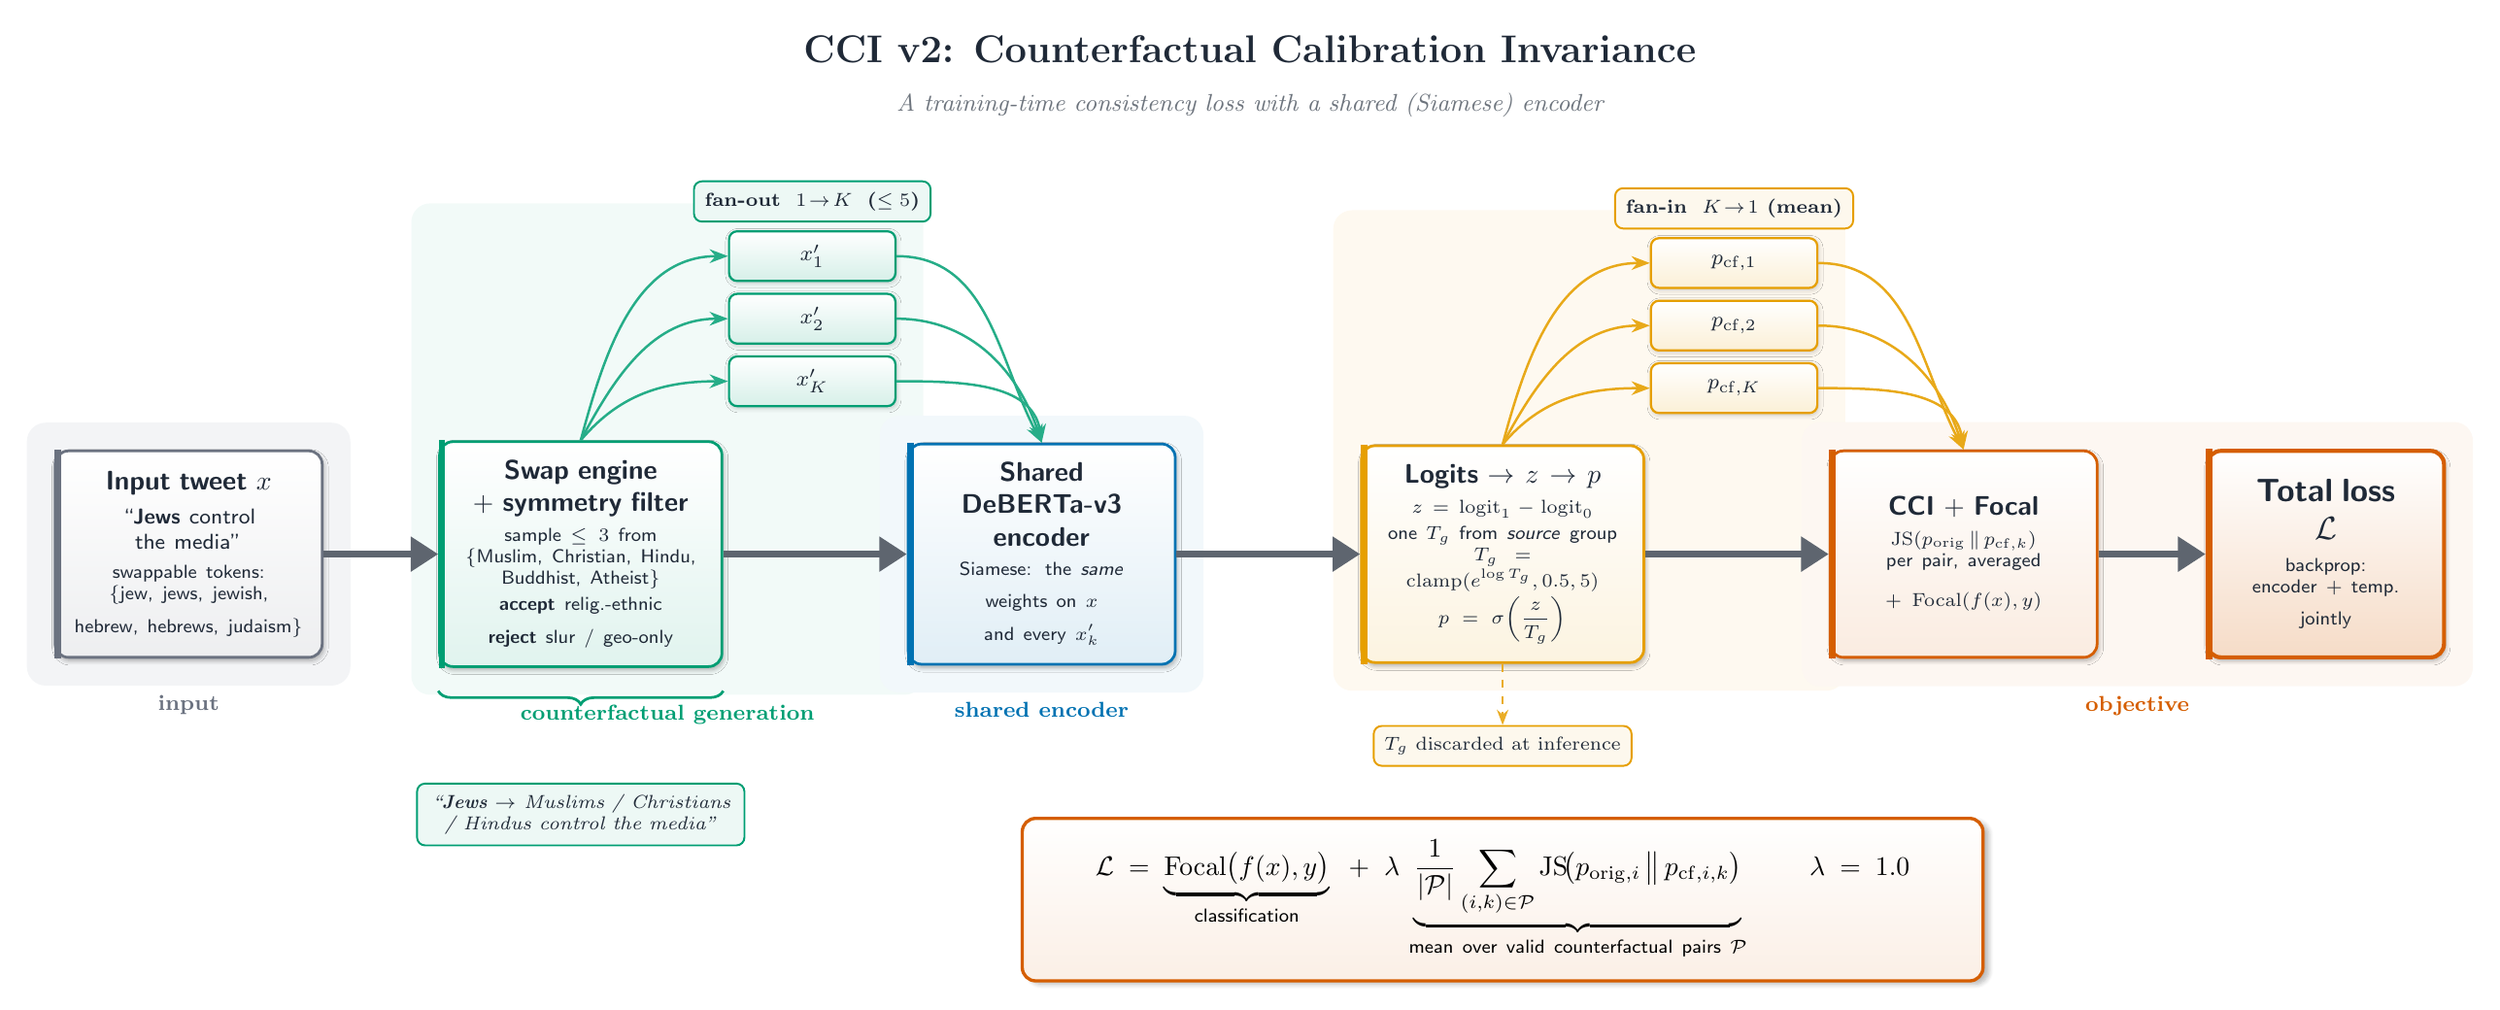
\begin{tikzpicture}[
  font=\sffamily,
  >={Stealth[round]},
  % ---- CARD: gradient fill + soft blur shadow + coloured accent via draw ----
  card/.style 2 args={
    rounded corners=5pt, draw=#1, line width=1pt,
    top color=white, bottom color=#1!12,
    blur shadow={shadow blur steps=6, shadow xshift=0.6pt,
                 shadow yshift=-1.2pt, shadow opacity=32},
    text=inkdark, align=center, inner sep=7pt,
    minimum height=27mm, text width=#2
  },
  % thin coloured accent strip drawn on a card's left edge
  accent/.style={line width=2.4pt, draw=#1},
  % small counterfactual / probability chips
  chip/.style={
    rounded corners=3pt, draw=#1, line width=0.8pt,
    top color=white, bottom color=#1!16, text=inkdark,
    inner sep=2.5pt, align=center, minimum height=6.5mm, text width=20mm,
    font=\footnotesize,
    blur shadow={shadow blur steps=4, shadow xshift=0.4pt,
                 shadow yshift=-0.7pt, shadow opacity=22}
  },
  note/.style={
    rounded corners=3pt, draw=#1, line width=0.7pt, fill=#1!7,
    text=inkdark, font=\scriptsize, inner sep=4pt, align=center
  },
  flow/.style={-{Triangle[length=3.6mm,width=4.4mm]},
               line width=2.4pt, draw=inkdark!72},
  fan/.style={-{Stealth[length=2.4mm]}, line width=0.9pt, draw=contribgreen!85},
  fin/.style={-{Stealth[length=2.4mm]}, line width=0.9pt, draw=tempgold!90},
]

% =====================================================================
%  MAIN ROW OF CARDS  (title added at the very end, above the bbox)
% =====================================================================
\node[card={inputgrey}{30mm}] (inp) at (0,0) {
  \textbf{Input tweet $x$}\\[3pt]
  \footnotesize ``\textbf{Jews} control\\the media''\\[3pt]
  \scriptsize swappable tokens:\\\{jew, jews, jewish,\\hebrew, hebrews, judaism\}
};

\node[card={contribgreen}{32mm}, right=15mm of inp] (swap) {
  \textbf{Swap engine}\\\textbf{$+$ symmetry filter}\\[3pt]
  \scriptsize sample $\le 3$ from\\\{Muslim, Christian, Hindu,\\Buddhist, Atheist\}\\[2pt]
  \scriptsize \textbf{accept} relig.-ethnic\\\textbf{reject} slur / geo-only
};

\node[card={encblue}{30mm}, right=24mm of swap] (enc) {
  \textbf{Shared}\\\textbf{DeBERTa-v3}\\\textbf{encoder}\\[3pt]
  \scriptsize Siamese: the \emph{same}\\weights on $x$ and every $x'_k$
};

\node[card={tempgold}{32mm}, right=24mm of enc] (prob) {
  \textbf{Logits $\to z \to p$}\\[3pt]
  \scriptsize $z=\mathrm{logit}_1-\mathrm{logit}_0$\\[2pt]
  \scriptsize one $T_g$ from \emph{source} group\\$T_g=\mathrm{clamp}(e^{\log T_g},0.5,5)$\\[2pt]
  $p=\sigma\!\left(\dfrac{z}{T_g}\right)$
};

\node[card={lossverm}{30mm}, right=24mm of prob] (js) {
  \textbf{CCI $+$ Focal}\\[3pt]
  \scriptsize $\mathrm{JS}(p_{\mathrm{orig}}\,\|\,p_{\mathrm{cf},k})$\\per pair, averaged\\[3pt]
  \scriptsize $+\;\mathrm{Focal}(f(x),y)$
};

\node[card={lossverm}{26mm}, right=14mm of js,
      bottom color=lossverm!22, line width=1.5pt] (loss) {
  \textbf{\large Total loss}\\[2pt]\textbf{\large $\mathcal{L}$}\\[4pt]
  \scriptsize backprop:\\encoder $+$ temp.\\jointly
};

% ---- left accent strips on each card (modern card look) ----
\foreach \n/\c in {inp/inputgrey, swap/contribgreen, enc/encblue,
                   prob/tempgold, js/lossverm, loss/lossverm}{
  \draw[accent=\c] ([xshift=1.4pt]\n.north west) -- ([xshift=1.4pt]\n.south west);
}

% =====================================================================
%  MAIN FLOW ARROWS
% =====================================================================
\draw[flow] (inp)  -- (swap);
\draw[flow] (swap) -- (enc);
\draw[flow] (enc)  -- (prob);
\draw[flow] (prob) -- (js);
\draw[flow] (js)   -- (loss);

% =====================================================================
%  FAN-OUT (1 -> K) above the swap->encoder gap
% =====================================================================
\node[chip={contribgreen}, above=14mm of enc, xshift=-30mm, yshift=7mm] (cf1){$x'_1$};
\node[chip={contribgreen}, below=1.4mm of cf1] (cf2){$x'_2$};
\node[chip={contribgreen}, below=1.4mm of cf2] (cf3){$x'_K$};
\draw[fan] (swap.north) to[out=75,in=180] (cf1.west);
\draw[fan] (swap.north) to[out=62,in=180] (cf2.west);
\draw[fan] (swap.north) to[out=50,in=180] (cf3.west);
\draw[fan] (cf1.east) to[out=0,in=118] (enc.north);
\draw[fan] (cf2.east) to[out=0,in=108] (enc.north);
\draw[fan] (cf3.east) to[out=0,in=98]  (enc.north);
\node[note={contribgreen}, above=1mm of cf1, font=\scriptsize\bfseries]
  {fan-out\; $1\!\to\!K$ \;($\le 5$)};

% =====================================================================
%  FAN-IN (K -> 1) above the prob->js gap
% =====================================================================
\node[chip={tempgold}, above=14mm of js, xshift=-30mm, yshift=7mm] (p1){$p_{\mathrm{cf},1}$};
\node[chip={tempgold}, below=1.4mm of p1] (p2){$p_{\mathrm{cf},2}$};
\node[chip={tempgold}, below=1.4mm of p2] (p3){$p_{\mathrm{cf},K}$};
\draw[fin] (prob.north) to[out=75,in=180] (p1.west);
\draw[fin] (prob.north) to[out=62,in=180] (p2.west);
\draw[fin] (prob.north) to[out=50,in=180] (p3.west);
\draw[fin] (p1.east) to[out=0,in=118] (js.north);
\draw[fin] (p2.east) to[out=0,in=108] (js.north);
\draw[fin] (p3.east) to[out=0,in=98]  (js.north);
\node[note={tempgold}, above=1mm of p1, font=\scriptsize\bfseries]
  {fan-in\; $K\!\to\!1$ (mean)};

% =====================================================================
%  CONTRIBUTION BRACE under the swap card
% =====================================================================
\draw[decorate, decoration={brace, amplitude=5pt, mirror},
      line width=1pt, draw=contribgreen]
  ([yshift=-3mm]swap.south west) -- ([yshift=-3mm]swap.south east)
  node[midway, below=6pt, font=\footnotesize\bfseries, text=contribgreen]
  {};

% worked example under the brace
\node[note={contribgreen}, below=15mm of swap, text width=40mm,
      font=\scriptsize\itshape] (ex){
  ``\textbf{Jews} $\to$ Muslims / Christians / Hindus control the media''
};

% "discarded at inference" callout under the temperature card
\node[note={tempgold}, below=8mm of prob, font=\scriptsize] (tnote)
  {$T_g$ discarded at inference};
\draw[-{Stealth[length=2mm]}, line width=0.8pt, draw=tempgold!85, dashed]
  (prob.south) -- (tnote.north);

% =====================================================================
%  LOSS EQUATION banner beneath the row
% =====================================================================
\node[rounded corners=5pt, draw=lossverm, line width=1.2pt,
      top color=white, bottom color=lossverm!10, inner sep=8pt,
      text width=120mm, align=center, below=20mm of prob,
      blur shadow={shadow blur steps=6, shadow yshift=-1.2pt, shadow opacity=28}]
      (eq){
  $\displaystyle
   \mathcal{L}=\underbrace{\mathrm{Focal}\big(f(x),y\big)}_{\text{classification}}
   \;+\;\lambda\,\underbrace{\frac{1}{|\mathcal{P}|}\sum_{(i,k)\in\mathcal{P}}
      \mathrm{JS}\!\big(p_{\mathrm{orig},i}\,\big\|\,p_{\mathrm{cf},i,k}\big)}_{\text{mean over valid counterfactual pairs }\mathcal{P}}$
  \qquad $\lambda=1.0$
};

% =====================================================================
%  PHASE-BAND BACKGROUNDS
% =====================================================================
\begin{scope}[on background layer]
  \node[fit=(inp), rounded corners=7pt, fill=bandgrey, inner sep=10pt,
        label={[font=\footnotesize\bfseries, text=inputgrey]below:input}] {};
  \node[fit=(swap)(cf1)(cf3), rounded corners=7pt, fill=contribgreen!5,
        inner sep=10pt,
        label={[font=\footnotesize\bfseries, text=contribgreen]below:counterfactual generation}] {};
  \node[fit=(enc), rounded corners=7pt, fill=encblue!5, inner sep=10pt,
        label={[font=\footnotesize\bfseries, text=encblue]below:shared encoder}] {};
  \node[fit=(prob)(p1)(p3), rounded corners=7pt, fill=tempgold!6, inner sep=10pt,
        label={[font=\footnotesize\bfseries, text=tempgold] below:}] {};
  \node[fit=(js)(loss), rounded corners=7pt, fill=lossverm!5, inner sep=10pt,
        label={[font=\footnotesize\bfseries, text=lossverm]below:objective}] {};
\end{scope}

% =====================================================================
%  TITLE  (added last so it sits above the full diagram, no collisions)
% =====================================================================
\node[font=\small\itshape, text=inkdark!65, anchor=south] (subt)
  at ([yshift=7mm]current bounding box.north)
  {A training-time consistency loss with a shared (Siamese) encoder};
\node[font=\bfseries\Large, text=inkdark, anchor=south] (maintitle)
  at ([yshift=1.5mm]subt.north)
  {CCI v2: Counterfactual Calibration Invariance};

\end{tikzpicture}
\end{document}
